\documentclass[10pt,handout]{beamer}

\usepackage[french]{babel}
\usepackage[utf8]{inputenc} 
\usepackage[T1]{fontenc}
\usepackage{lmodern}
\usepackage{beamerthemebars}
\usepackage{multicol}
\usepackage{pythontex}
\usepackage{amsmath}
\usepackage{graphics}
\usepackage{hyperref}
\usepackage{multimedia}
\usepackage{tikz}
\usetikzlibrary{calc}
\usetikzlibrary{fpu}
\usetikzlibrary{arrows.meta}
\usetikzlibrary{angles,quotes}
\usetikzlibrary{decorations.pathmorphing,patterns}
\usetikzlibrary{datavisualization.formats.functions}
%\usepackage[french]{babel}
\usepackage{pgfplots}
\pgfplotsset{compat=1.15}
\usepackage{mathrsfs}
\usetikzlibrary{arrows}
\usepackage{latexsym} % Símbolos                        ı
\usepackage{amsmath}
\usepackage{amssymb}
%%%%%%%%%%%%%%%%%%%%%%%%%%%%%%%
\usepackage{tikz-3dplot}
\usepackage[outline]{contour} % glow around text
\usepackage{xcolor}
\usepackage{listings}

\definecolor{codegreen}{rgb}{0,0.6,0}
\definecolor{codegray}{rgb}{0.5,0.5,0.5}
\definecolor{codepurple}{rgb}{0.58,0,0.82}
\definecolor{backcolour}{rgb}{0.95,0.95,0.92}

\lstdefinestyle{mystyle}{
    backgroundcolor=\color{backcolour},   
    commentstyle=\color{codegreen},
    keywordstyle=\color{magenta},
    numberstyle=\tiny\color{codegray},
    stringstyle=\color{codepurple},
    basicstyle=\ttfamily\footnotesize,
    breakatwhitespace=false,         
    breaklines=true,                 
    captionpos=b,                    
    keepspaces=true,                 
    numbers=left,                    
    numbersep=5pt,                  
    showspaces=false,                
    showstringspaces=false,
    showtabs=false,                  
    tabsize=2
}

\lstset{style=mystyle}

\colorlet{veccol}{green!50!black}
\colorlet{projcol}{blue!70!black}
\colorlet{myblue}{blue!80!black}
\colorlet{myred}{red!90!black}
\colorlet{mydarkblue}{blue!50!black}
\tikzset{>=latex} % for LaTeX arrow head
\tikzstyle{proj}=[projcol!80,line width=0.08] %very thin
\tikzstyle{area}=[draw=veccol,fill=veccol!80,fill opacity=0.6]
\tikzstyle{vector}=[-stealth,myblue,thick,line cap=round]
\tikzstyle{unit vector}=[->,veccol,thick,line cap=round]
\tikzstyle{dark unit vector}=[unit vector,veccol!70!black]
\usetikzlibrary{angles,quotes} % for pic (angle labels)
\contourlength{1.3pt}

%%%%%%%%%%%%%%%%%%%%%%%%%%%%%%%
\theoremstyle{plain} % default
  \newtheorem{thm}{Th\'eor\`eme}
\theoremstyle{definition}
  \newtheorem{defn}{D\'efinition}
\theoremstyle{example}
  \newtheorem{exmp}{Exemple}
\theoremstyle{example}
  \newtheorem{problema}{Probl\'eme}
\theoremstyle{remark}
  \newtheorem{respuesta}{R\'eponse}
\theoremstyle{remark}
  \newtheorem{rem}{Note}
%%%%%%%%%%%%%%%%%%%%%%%%%%%%
%\frenchdecimal{.}
%\useoutertheme{infolines}
%\usetheme{Marburg}
\setbeamercovered{transparent}

\title{Introducción al procesado de imagen digital}
\author{Antonio Falc\'o y Juan Pardo}
\date{Introducción a la Inteligencia Artificial} 

\begin{document}

\frame[plain]{%
\maketitle
}

%\begin{frame}
%  \tableofcontents
%\end{frame}

%\section{Contexto}
\frame[plain]{%
  \frametitle{Aprendizaje}  
  \framesubtitle{Una breve introducción al concepto de aprendizaje y a la inteligencia artificial en el campo del diseño de producto y de los procesos de fabricación.}
  \begin{block}{El proceso de aprendizaje}
    El aprendizaje es el proceso de adquisición de conocimientos, habilidades y actitudes a través de la experiencia, la instrucción y el estudio.
  \end{block}
  \begin{block}{El aprendizaje en la inteligencia artificial}
    En el campo de la inteligencia artificial, el aprendizaje es el proceso de \textcolor{red}{entrenar con un ordenador un modelo matemático  alimentado con datos para realizar una tarea específica}, como reconocer patrones en datos, tomar decisiones o predecir resultados.
\end{block}
\begin{block}{El proceso de aprendizaje con imágenes digitales}
  En el campo del procesamiento de imágenes digitales, el aprendizaje es el proceso de \textcolor{red}{entrenar con un ordenador un modelo matemático  alimentado con datos para analizar y procesar imágenes digitales}, como reconocer objetos, segmentar regiones de interés o mejorar la calidad de las imágenes.
\end{block}
%\py{2+2}
}

\frame[plain]{%
  \frametitle{Aprendizaje}  
  \framesubtitle{El esquema del proceso de aprendizaje máquina.}
\begin{center}
  \begin{tikzpicture}
    \node[draw] at (0,1) {\textcolor{blue}{Entrenamiento = Aprendizaje}};
    \node (A) at (0,0) {Datos = (Imágenes,Etiquetas)};
    \node[draw] (B) at (-6,-0.8) {\textcolor{red}{Modelo}};
    \node (C) at (-4,-0.8) {Imágenes};
    \node (D) at (0,-0.8) {Etiquetas};
    \node (E) at (-4,-3) {Imágenes};
    \node (F) at (0,-3) {Etiquetas};
    \node at (-5,-0.8) {$\times$};
    \draw[<-] (A)  (B) (D) -- (C);
    \node[draw] at (-2,-1.5) {\textcolor{red}{Procedimiento = Algoritmo}};
    \node[draw] at (0,-2.3) {\textcolor{blue}{Modelo Entrenado}};
    \draw[->] (E) -- (F);
  \end{tikzpicture}
\end{center}
\begin{itemize}
\item El proceso de \textcolor{blue}{aprendizaje = entrenamiento} lleva consigo la construcción de un modelo matemático que es alimentado con datos (imágenes y etiquetas) para realizar una tarea específica, como reconocer objetos en imágenes, segmentar regiones de interés o mejorar la calidad de las imágenes. 
\item La construcción del modelo se realiza empleando un \textcolor{red}{procedimiento = algoritmo}.
\end{itemize}
}

\frame[plain]{%
  \frametitle{Problemas clave}  
  %\framesubtitle{}
\centering
  \begin{enumerate}
    \item \textbf{Representación de datos}: La representación de datos es un desafío importante, ya que los \textcolor{red}{datos} pueden ser complejos y difíciles de analizar.
    
    \item \textbf{Optimización}: La optimización es un problema clave en la inteligencia artificial, ya que muchos \textcolor{red}{algoritmos} buscan encontrar las mejores soluciones entre múltiples opciones.

    \item \textbf{Escalabilidad}: La escalabilidad se refiere a la capacidad de los \textcolor{red}{algoritmos} para manejar grandes cantidades de datos y hacer predicciones precisas en tiempo real.

    \item \textbf{Interpretabilidad}: La interpretabilidad es el problema de entender cómo los \textcolor{red}{algoritmos} llegan a sus conclusiones y por qué toman ciertas decisiones.

    \item \textbf{Robustez}: La robustez se refiere a la capacidad de los \textcolor{red}{algoritmos} para funcionar correctamente en diferentes condiciones y ambientes.

    \item \textbf{Explicabilidad}: La explicabilidad es el problema de justificar las decisiones tomadas por los \textcolor{red}{algoritmos} y cómo se relacionan con los \textcolor{red}{datos} de entrada.
  
    \item \textbf{Equidad}: La equidad se refiere a la capacidad de los \textcolor{red}{algoritmos} para tomar decisiones no discriminatorias y respetuosas con los derechos humanos.
  \end{enumerate}
}

\frame[plain]{%
  \frametitle{Introducción al procesado de imagen digital} 
\begin{itemize}
\item En el mundo digital, las imágenes son una forma fundamental de comunicar información y transmitir conocimientos. Sin embargo, para que un ordenador pueda procesar y manipular estas imágenes, es necesario convertirlas en un formato numérico que sea comprensible por el dispositivo. Esta codificación numérica se conoce como representación numérica de las imágenes.

\item La representación numérica de las imágenes implica asignar valores numéricos a cada píxel (unidad básica de la imagen) que contenga información sobre su color, intensidad y posición en la imagen. De esta manera, el ordenador puede analizar y manipular los píxeles individualmente, lo que abre la puerta a una amplia gama de posibilidades para la procesamiento de imágenes.

\end{itemize}
}


\frame[plain]{%
  \frametitle{Introducción al procesado de imagen digital} 
\begin{itemize}
\item La representación numérica de las imágenes es fundamental para aplicaciones como la visión por computadora, el reconocimiento facial, la detección de objetos y la generación de gráficos. Además, esta representación es crítica en campos como la medicina, donde se utilizan imágenes médicas para diagnosticar enfermedades o seguir el progreso del paciente.

\item En este contexto, es importante entender cómo las imágenes se convierten en un formato numérico que sea manipulable por el ordenador y cómo se pueden manipular estos valores numéricos para lograr diferentes efectos.
\end{itemize}
}

\frame[plain]{%
  \frametitle{Introducción al procesado de imagen digital}  
  \framesubtitle{Una breve revisión de la tećnicas de procesado de imagen digital y al tratamiento de imágenes digitales como datos numéricos.}
  \begin{block}{Codificación de imágenes}
    Las imágenes digitales se componen de píxeles, que son los elementos más pequeños de una imagen. Cada píxel tiene un valor numérico que representa su color o intensidad.
  \end{block}
  \begin{block}{Representación numérica de imágenes digitales}
    Las imágenes digitales se pueden representar como matrices de píxeles, donde cada píxel tiene un valor numérico que representa su color o intensidad.
\end{block}
\begin{block}{Manipulación numérica de imágenes digitales}
  Las imágenes digitales se pueden manipular utilizando técnicas de procesamiento de imágenes, como la convolución, la transformación de Fourier y la segmentación.
\end{block}
}

\frame[plain]{%
  \frametitle{¿Qué es una imagen?}
  \centering
  \framesubtitle{Proyección de un objeto sobre la retina}
  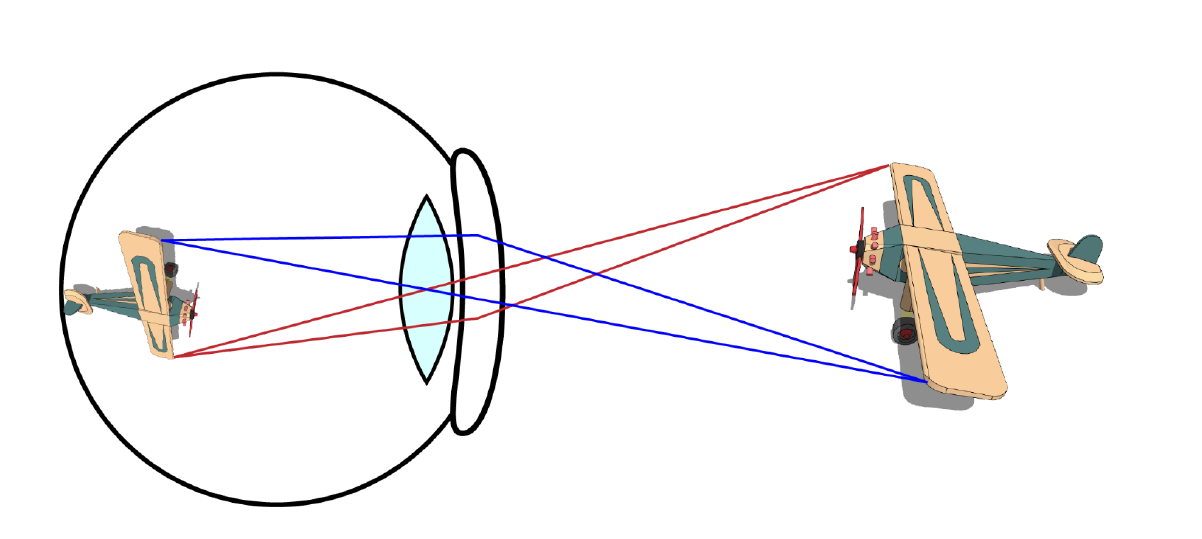
\includegraphics[width=0.8\textwidth]{./imagen1.png}
}

\frame[plain]{%
  \frametitle{¿Qué es una imagen?}
  \centering
  \framesubtitle{Modelo: Cámara de aguja}
  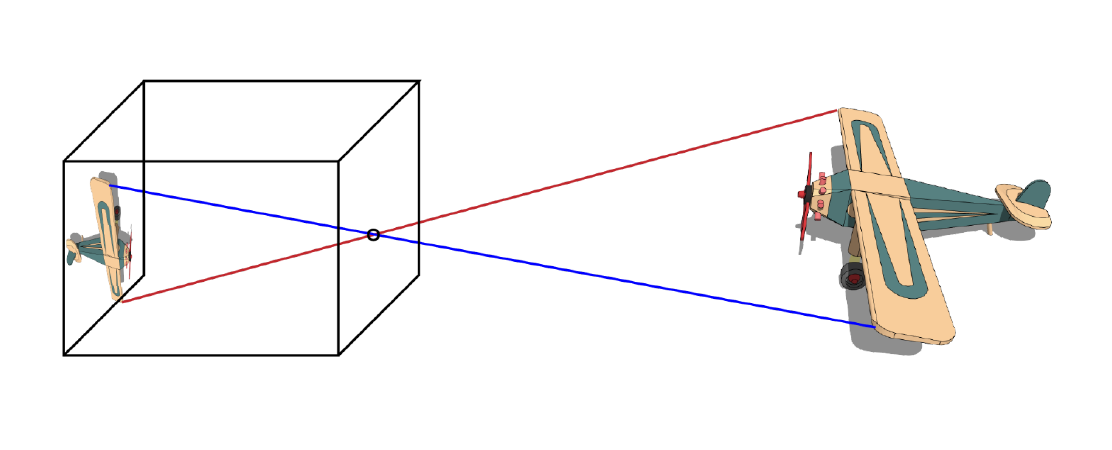
\includegraphics[width=0.8\textwidth]{./imagen2.png}
}

\frame[plain]{%
  \frametitle{¿Qué es una imagen?}
  \centering
  \framesubtitle{Modelo: Cámara de aguja}
  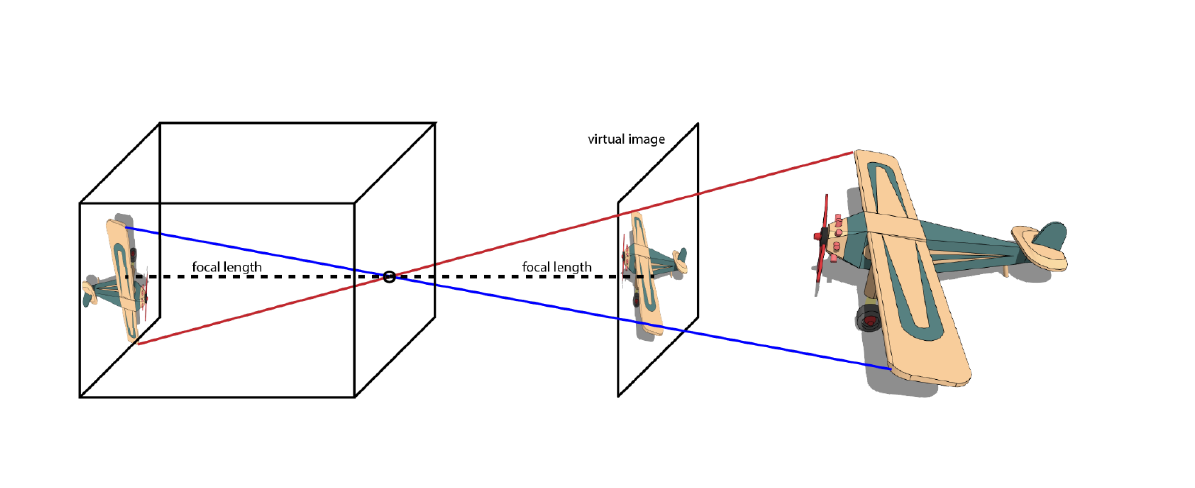
\includegraphics[width=0.8\textwidth]{./imagen3.png}
}

\frame[plain]{%
  \frametitle{¿Qué es una imagen?}
  \centering
  \framesubtitle{En cada punto grabamos la luz incidente en la cámara}
  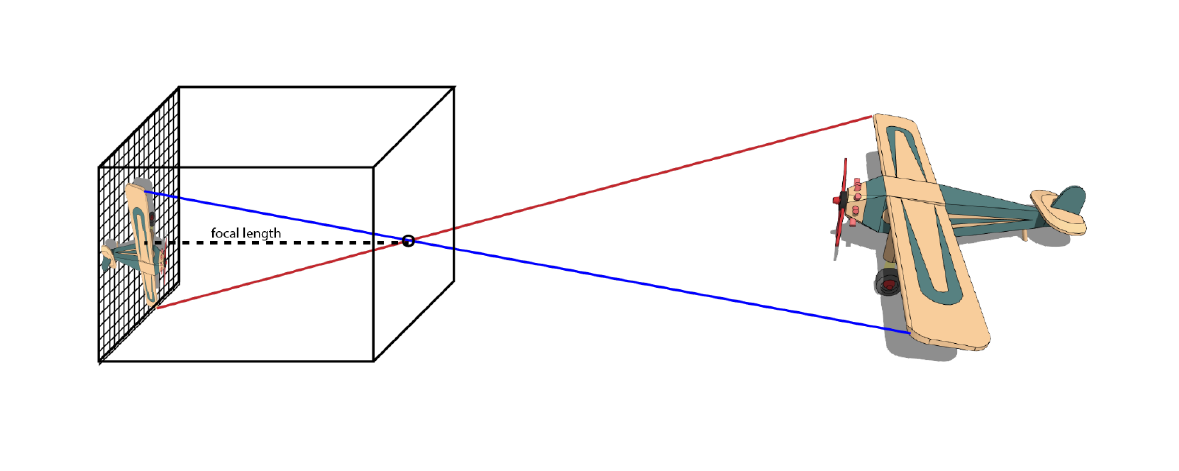
\includegraphics[width=0.8\textwidth]{./imagen4.png}
}

\frame[plain]{%
  \frametitle{¿Qué es una imagen?}
  \centering
  \framesubtitle{Una imagen es una matriz de luz}
  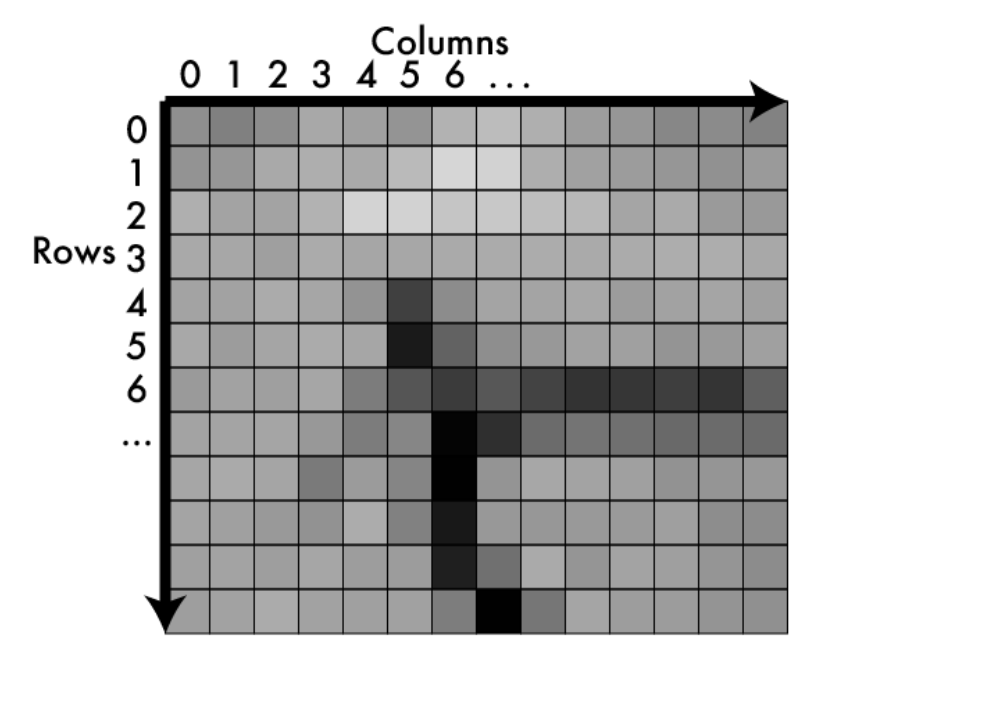
\includegraphics[width=0.8\textwidth]{./imagen5.png}
}

\frame[plain]{%
  \frametitle{¿Qué es una imagen?}
  \centering
  \framesubtitle{Los valores en la matriz = intensidad de luz}
  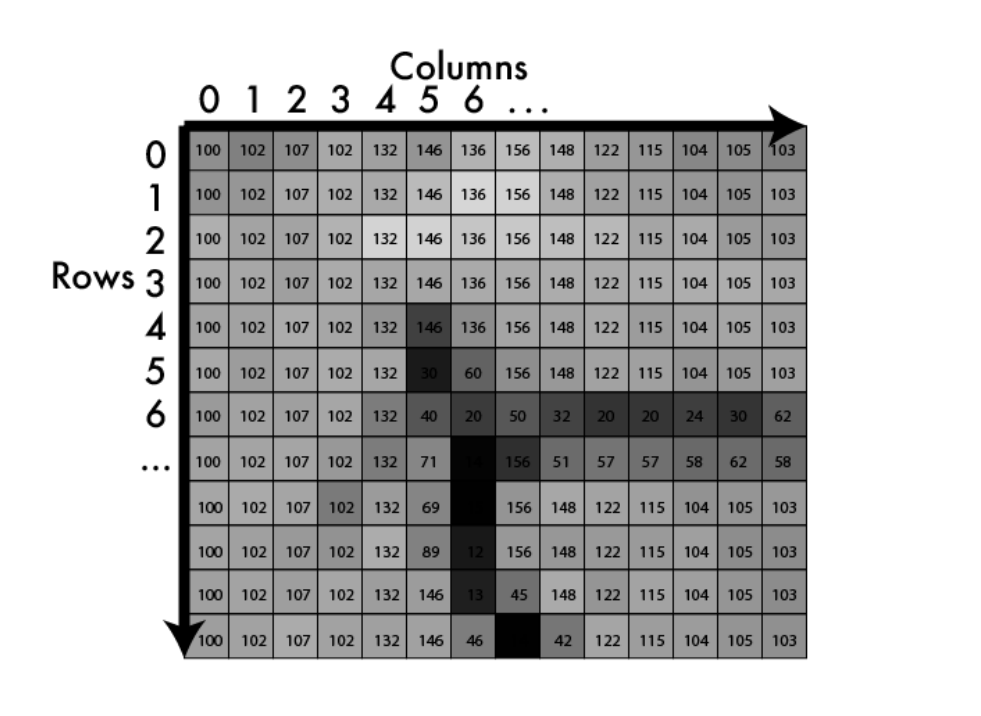
\includegraphics[width=0.8\textwidth]{./imagen6.png}
}

\frame[plain]{%
  \frametitle{¿Qué es una imagen?}
  \framesubtitle{Codificación de la intensidad de luz}
  
  La matriz asociada a una imagen digital se codifica utilizando un formato de archivo específico y una representación numérica de los píxeles.

  Los formatos comunes para codificar matrices de imágenes digitales son:
  \begin{itemize}
  
      \item \textbf{RAW}: El formato RAW es un formato no procesado que almacena los valores de los píxeles en un formato binario. Cada pixel se representa como un entero sin signo entre 0 y 65535 $( = 2^{16}-1)$.
  
      \item \textbf{Bitmap (BMP)}: El formato BMP es un formato de archivo que almacena las matrices de imágenes digitales utilizando una representación de píxeles en formato RGB (Red, Green, Blue). Cada pixel se representa como un valor entre 0 y 255 $=(2^8-1)$ para cada componente de color.

  \end{itemize} 
}

\frame[plain]{%
  \frametitle{¿Qué es una imagen?}
  \framesubtitle{Codificación de la intensidad de luz}
  
  La matriz asociada a una imagen digital se codifica utilizando un formato de archivo específico y una representación numérica de los píxeles.

  Los formatos comunes para codificar matrices de imágenes digitales son:
  \begin{itemize}
  
  
      \item \textbf{JPEG}: El formato JPEG (Joint Photographic Experts Group) es un formato de archivo que utiliza una compresión predictiva para reducir el tamaño del archivo. La matriz asociada a la imagen se codifica en forma de cuadrícula, donde cada pixel se representa como un valor entre 0 y 255.
  
      \item \textbf{PNG}: El formato PNG (Portable Network Graphics) es un formato de archivo que utiliza una compresión sin pérdida para reducir el tamaño del archivo. La matriz asociada a la imagen se codifica en forma de cuadrícula, donde cada pixel se representa como un valor entre 0 y 255.
  \end{itemize} 
}



\frame[plain]{%
  \frametitle{¿Qué es una imagen?}
  \framesubtitle{Codificación de la intensidad de luz}

  En cuanto a la representación numérica de los píxeles, las matrices de imágenes digitales suelen ser representadas utilizando valores enteros o flotantes. Los valores más comunes son:
  
  \begin{enumerate}
      \item Enteros: Los valores de los píxeles se representan como enteros sin signo entre 0 y 255 (8 bits) o entre 0 y 65535 (16 bits).
  
      \item Coma flotante: Los valores de los píxeles se representan como números reales en coma flotante en un rango determinado, generalmente entre 0 y 1.
  
  \end{enumerate}
  En resumen, la matriz asociada a una imagen digital se codifica utilizando un formato de archivo específico y una representación numérica de los píxeles. Los formatos más comunes son RAW, BMP, JPEG y PNG, mientras que las representaciones numéricas más comunes son enteros o flotantes.
}

\frame[plain]{%
  \frametitle{¿Qué es una imagen?}
  \framesubtitle{Indexación de píxeles}
  \begin{columns}
    
    \column{0.6\textwidth}
    \begin{itemize}
      \item Formas de indexación de píxeles en una imagen digital.
      \begin{itemize}
        \item $(\text{fila},\text{columna})$
        \begin{itemize}
          \item Índices de fila y columna.
          \item $(3,6)$ es la posición de un píxel en la fila 3 columna 6.
          \end{itemize}
        \item $(\text{coordenada h.},\text{coordenada v.})$
        \begin{itemize}
          \item Empleando coordenadas cartesianas $(x,y),$ pero con el origen en la esquina superior izquierda.
          \item $(3,6)$ es la posición de un píxel en la fila 3 columna 6.
          \end{itemize}
      \end{itemize}
    \end{itemize}
    
    \column{0.6\textwidth}
    \centering
  
  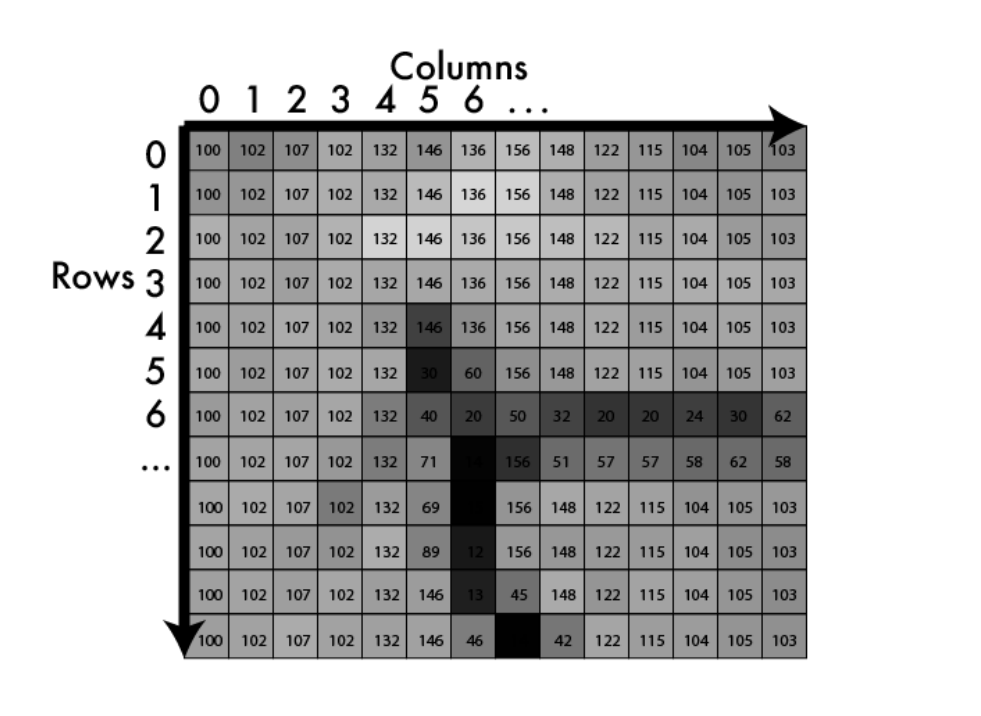
\includegraphics[width=0.9\textwidth]{./imagen6.png}

    \end{columns}
}

\frame[plain]{%
  \frametitle{¿Qué es una imagen?}
  \framesubtitle{Representación matemática de una imagen digital}

$$
\text{Imagen} = \begin{bmatrix}
  f(0,0) & f(0,1) & \cdots & f(0,H-1) \\
  f(1,0) & f(1,1) & \cdots & f(1,H-1) \\
  \vdots & \vdots & \ddots & \vdots \\
  f(W-1,0) & f(W-1,1) & \cdots & f(W-1,H-1) \\
\end{bmatrix}
$$
Se escribe de forma genérica $f(x,y),$ donde $x$ es la coordenada horizontal y $y$ es la coordenada vertical. $W$ es el ancho de la imagen y $H$ es la altura de la imagen. Matemáticamente, se representa como:
$$
f: \{0,1,\ldots,W-1\} \times \{0,1,\ldots,H-1\} \longrightarrow \mathbb{R}
$$
}

\frame[plain]{%
  \frametitle{¿Qué es una imagen?}
  \framesubtitle{¿Cómo se almacena una imagen en el ordenador?: Ejemplo}  
    \centering
  
  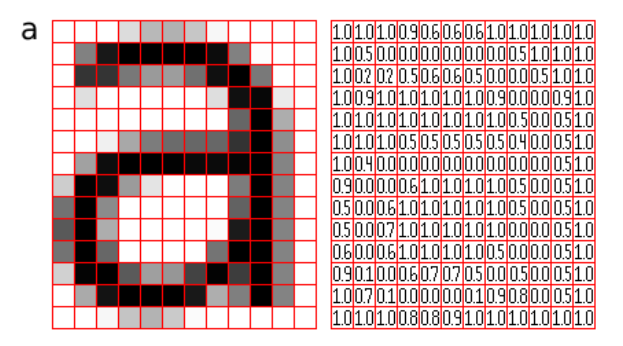
\includegraphics[width=0.9\textwidth]{./imagen19.png}

}

\frame[plain]{%
  \frametitle{¿Qué es una imagen?}
  \centering
  \framesubtitle{Imagen en color: Tensor 3d en el espacio RGB}
  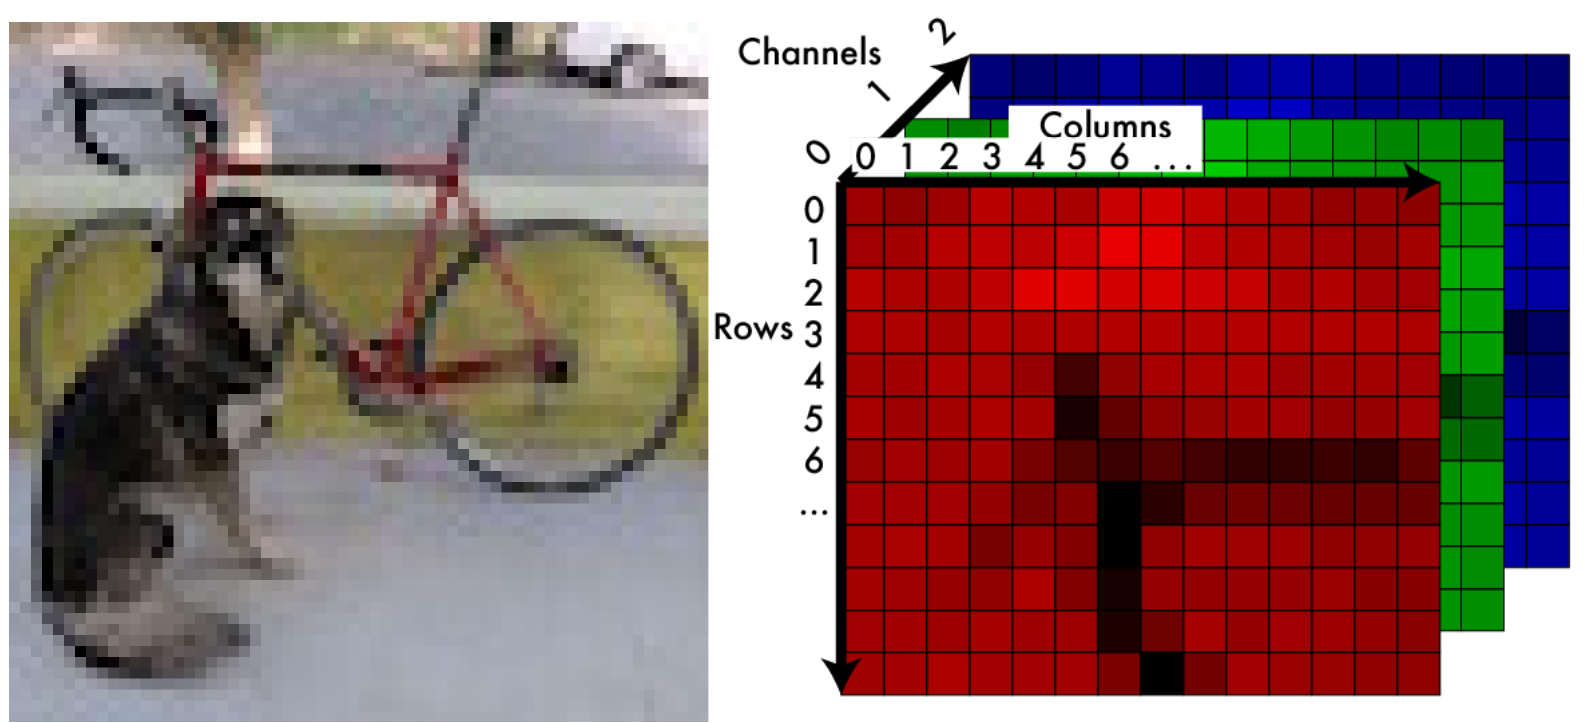
\includegraphics[width=0.9\textwidth]{./imagen7.png}
}

\frame[plain]{%
\frametitle{¿Qué es una imagen?}
\framesubtitle{Información RGB en "canales" separados}
  \begin{columns}  
    \column{0.6\textwidth}
    \begin{itemize}
      \item  Podemos sincronizar "colores reales" utilizando un mezcla de colores primarios
          \item Cada canal codifica un color
          primario. Agregar la luz producida a partir de cada primario imita el color original.
    \end{itemize}
    
    \column{0.6\textwidth}
    \centering
  
  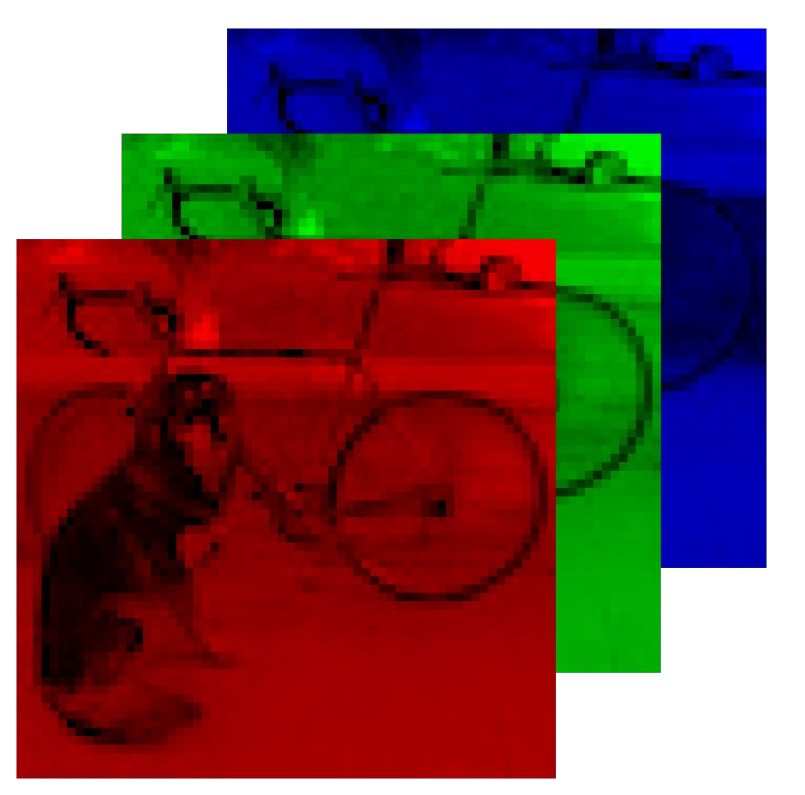
\includegraphics[width=0.9\textwidth]{./imagen8.png}

    \end{columns}
}

\frame[plain]{%
  \frametitle{¿Qué es una imagen?}
  \framesubtitle{Indexación de píxeles}
  \begin{columns}
    
    \column{0.6\textwidth}
    \begin{itemize}
      \item Formas de indexación de píxeles en una imagen digital.
      \begin{itemize}
        \item $(x,y,\text{color})$
        \begin{itemize}
          \item $(1,2,0)$ es la posición de un píxel en la fila 1 columna 2 del canal 0.
          \end{itemize}
      \end{itemize}
      \end{itemize}
    
    \column{0.6\textwidth}
    \centering
  
  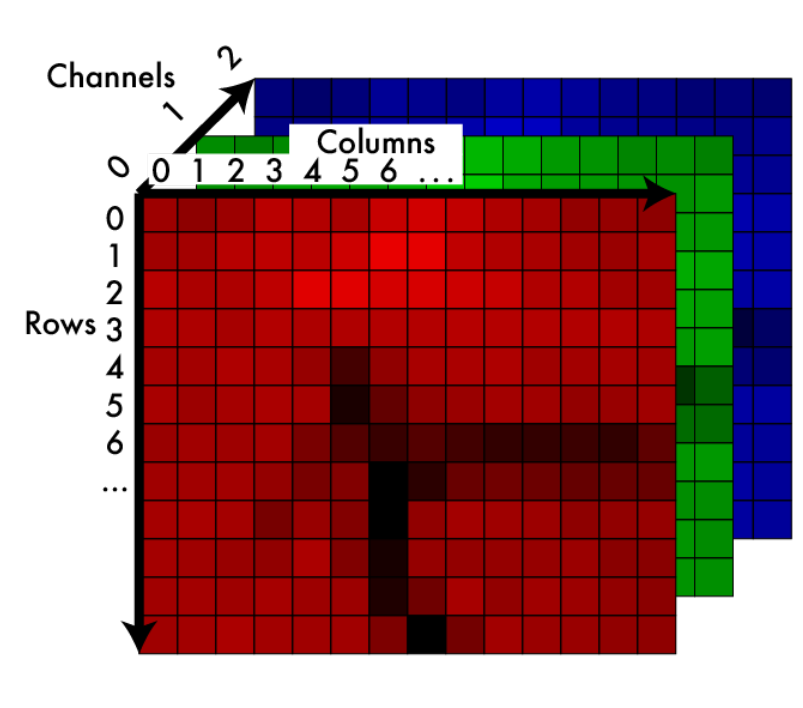
\includegraphics[width=0.9\textwidth]{./imagen9.png}

    \end{columns}
}

\frame[plain]{%
  \frametitle{¿Qué es una imagen?}
  \centering
  \framesubtitle{¿Cómo se almacena una imagen en el ordenador?}
  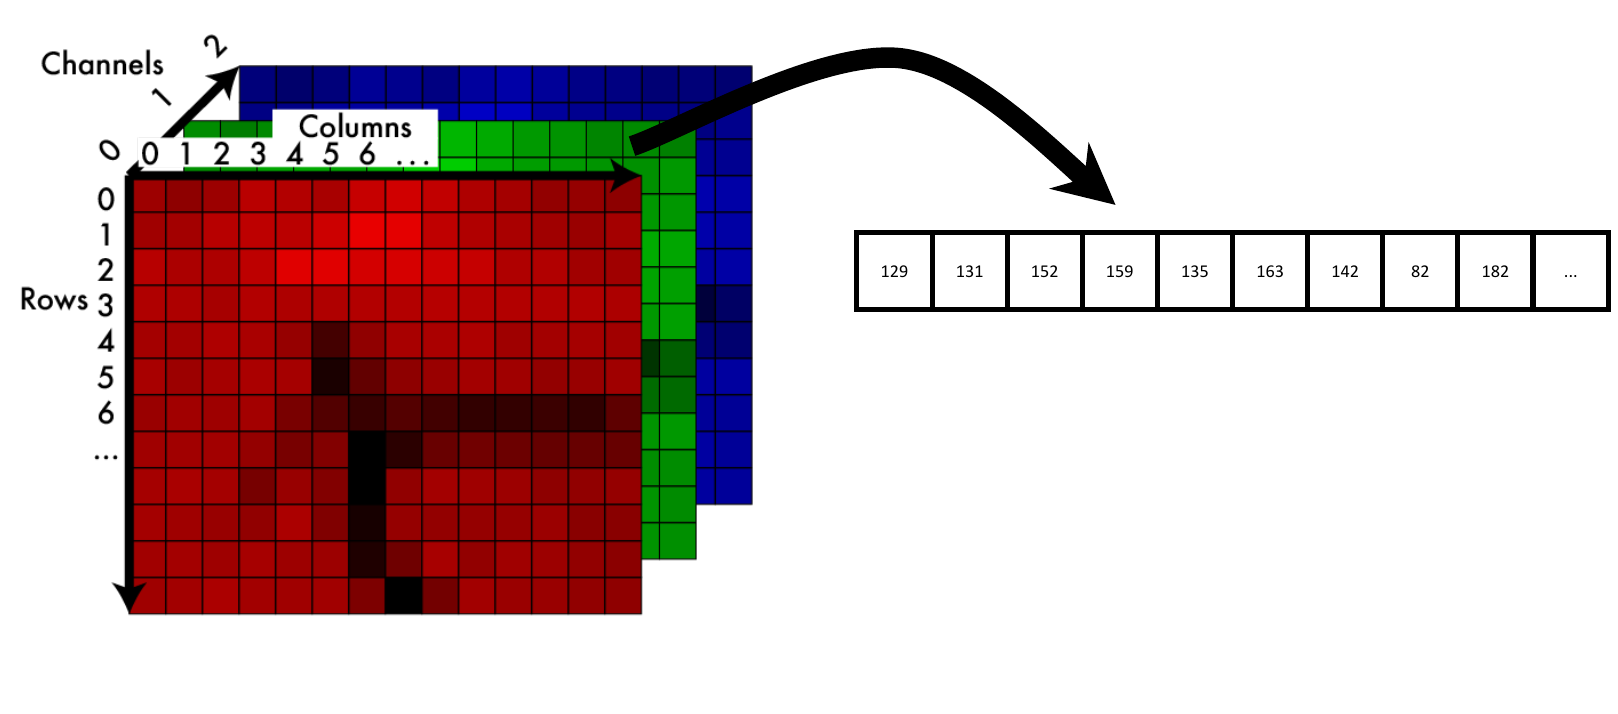
\includegraphics[width=1.2\textwidth]{./imagen10.png}
}


\frame[plain]{%
  \frametitle{¿Qué es una imagen?}
  \framesubtitle{¿Cómo se almacena una imagen en el ordenador?}

$$
\text{Imagen} = \begin{bmatrix}
  f(0,0) & f(0,1) & \cdots & f(0,H-1) \\
  f(1,0) & f(1,1) & \cdots & f(1,H-1) \\
  \vdots & \vdots & \ddots & \vdots \\
  f(W-1,0) & f(W-1,1) & \cdots & f(W-1,H-1) \\
\end{bmatrix}
$$
Se almacena en un \textcolor{red}{array = vector} de tamaño $W \times H$ donde $W$ es el ancho de la imagen, $H$ es la altura de la imagen
$$
\begin{bmatrix}
  f(0,0) & \cdots & f(0,H-1) 
  f(1,0) & \cdots
  f(1,H-1) &\cdots & f(W-1,H-1)
\end{bmatrix}
$$
}

\frame[plain]{%
  \frametitle{¿Qué es una imagen?}
  \centering
  \framesubtitle{Almacenamiento: Por filas vs. Por columnas}
  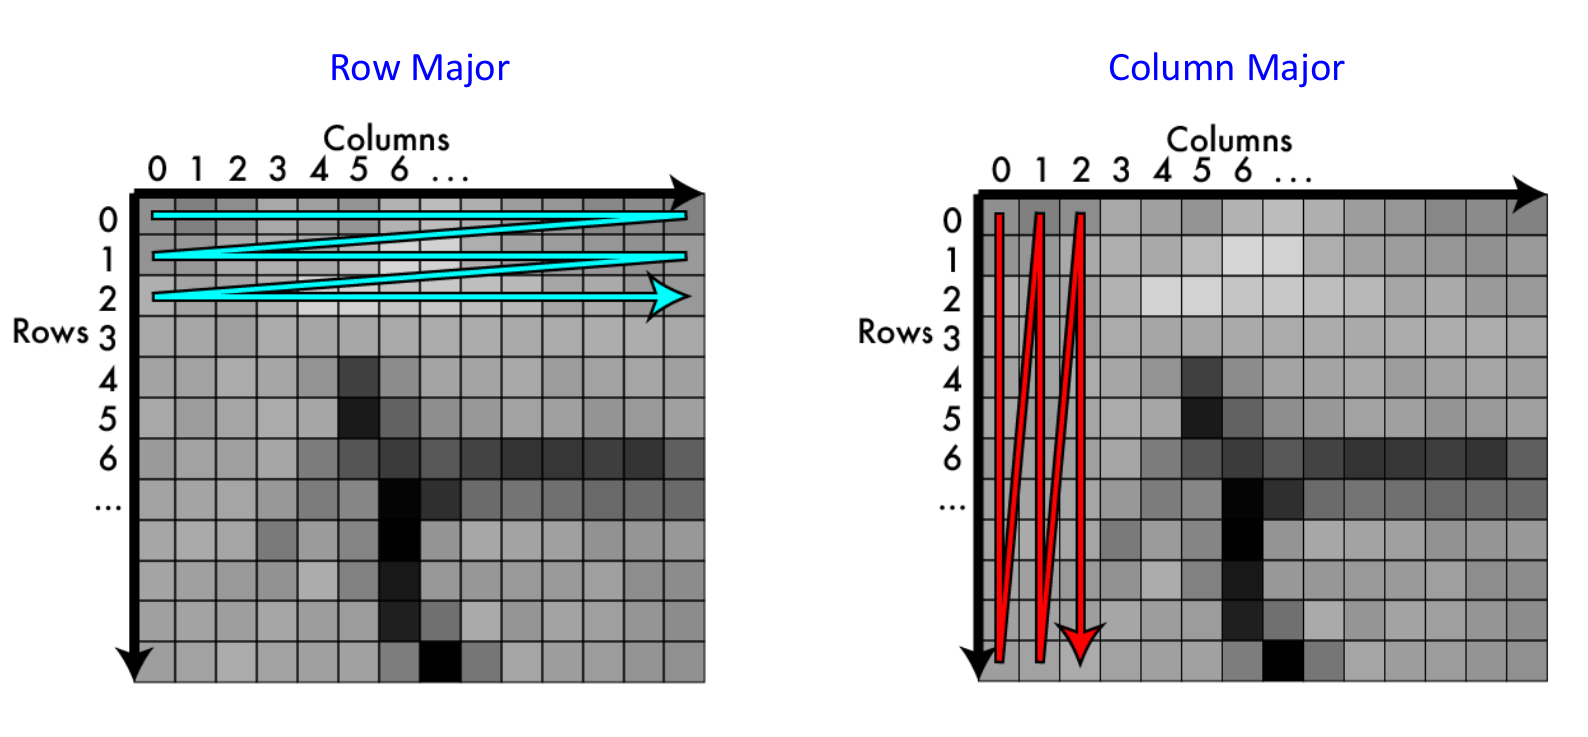
\includegraphics[width=1\textwidth]{./imagen11.png}
}

\frame[plain]{%
  \frametitle{¿Qué es una imagen?}
  \centering
  \framesubtitle{Tipicamente se emplea el almacenamiento por filas}
  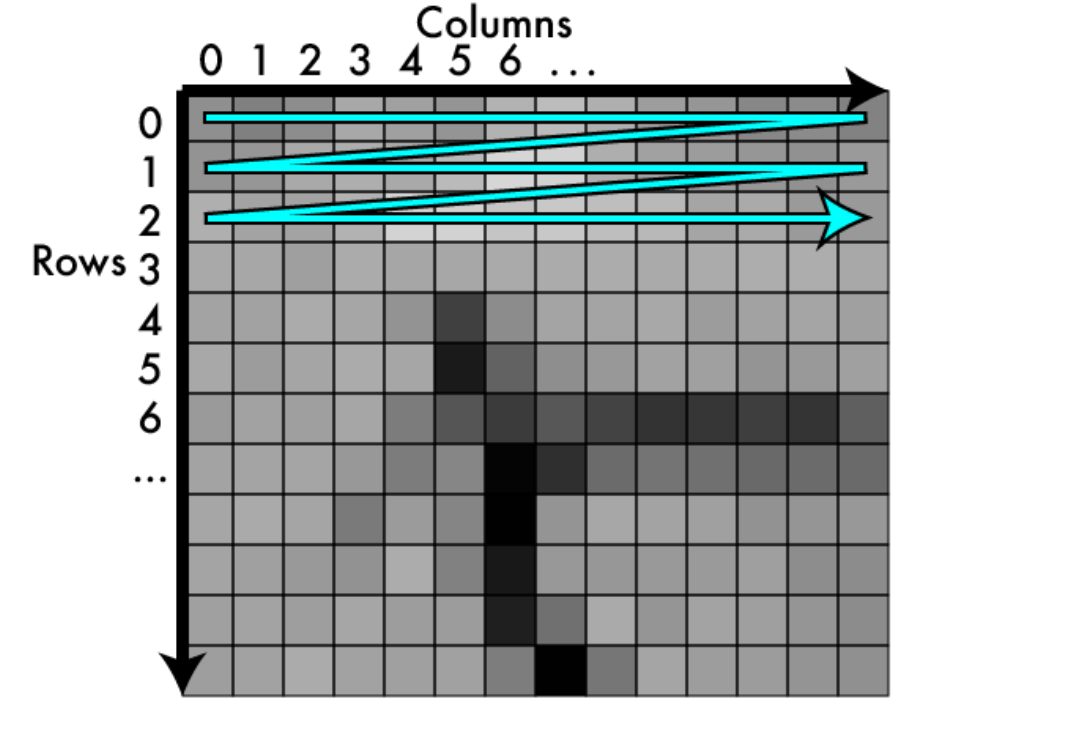
\includegraphics[width=1\textwidth]{./imagen12.png}
}

\frame[plain]{%
  \frametitle{¿Qué es una imagen?}
  \centering
  \framesubtitle{HWC: Height, Width, Channels (Alto, Ancho, Canales) Canales Intercalados} 
  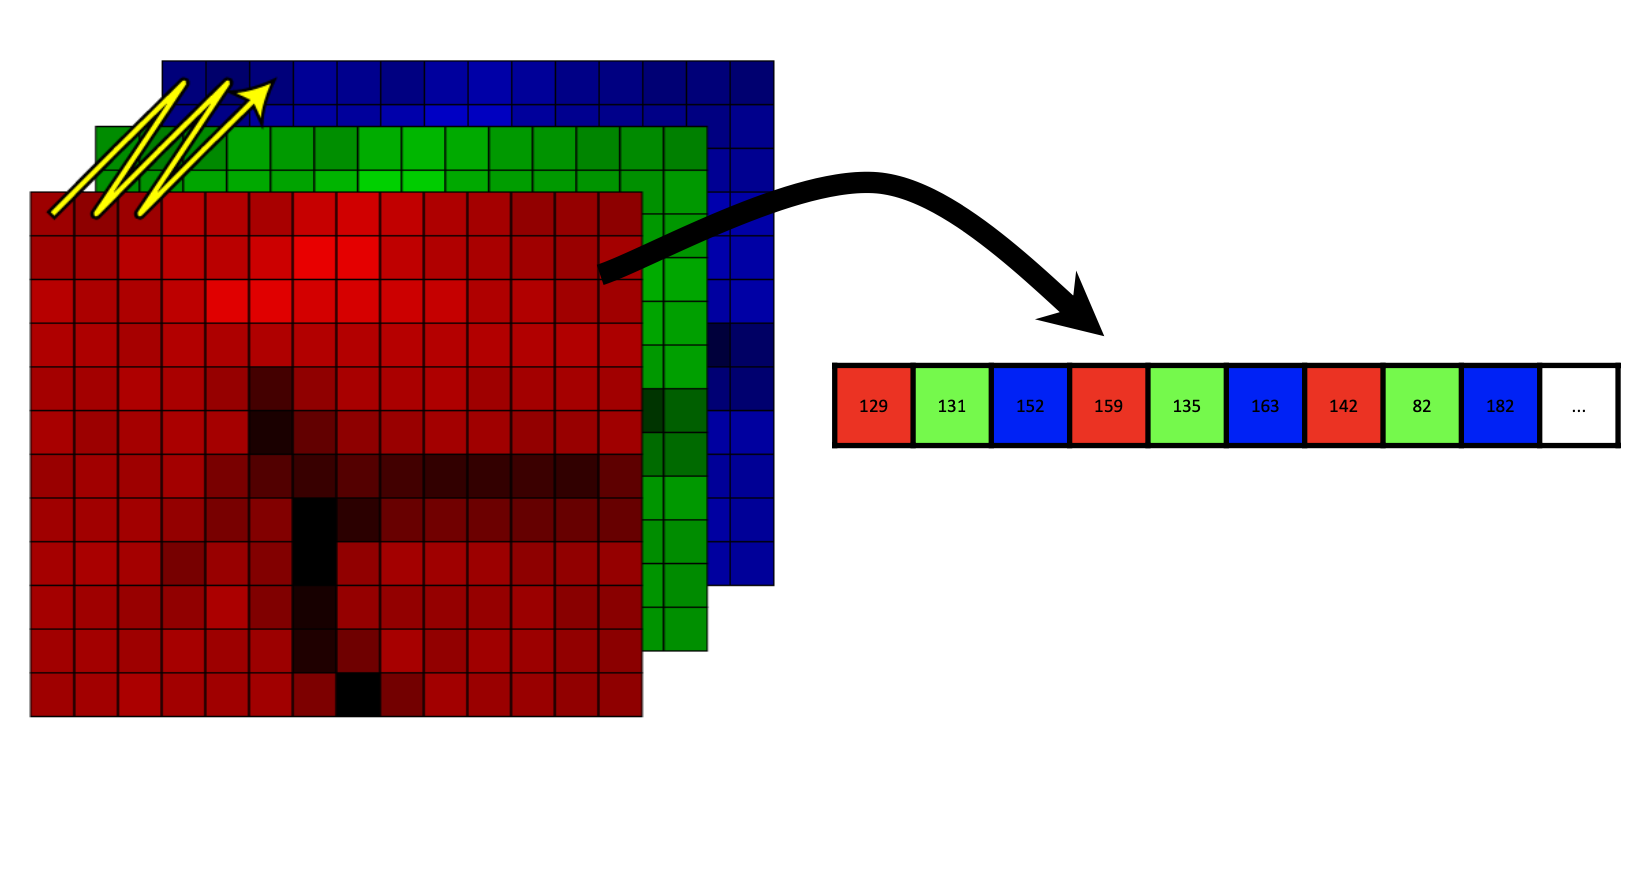
\includegraphics[width=1.2\textwidth]{./imagen13.png}
}

\frame[plain]{%
  \frametitle{¿Qué es una imagen?}
  \centering
  \framesubtitle{CHW: Channels, Height, Width  (Canales, Alto, Ancho) Canales Separados} 
  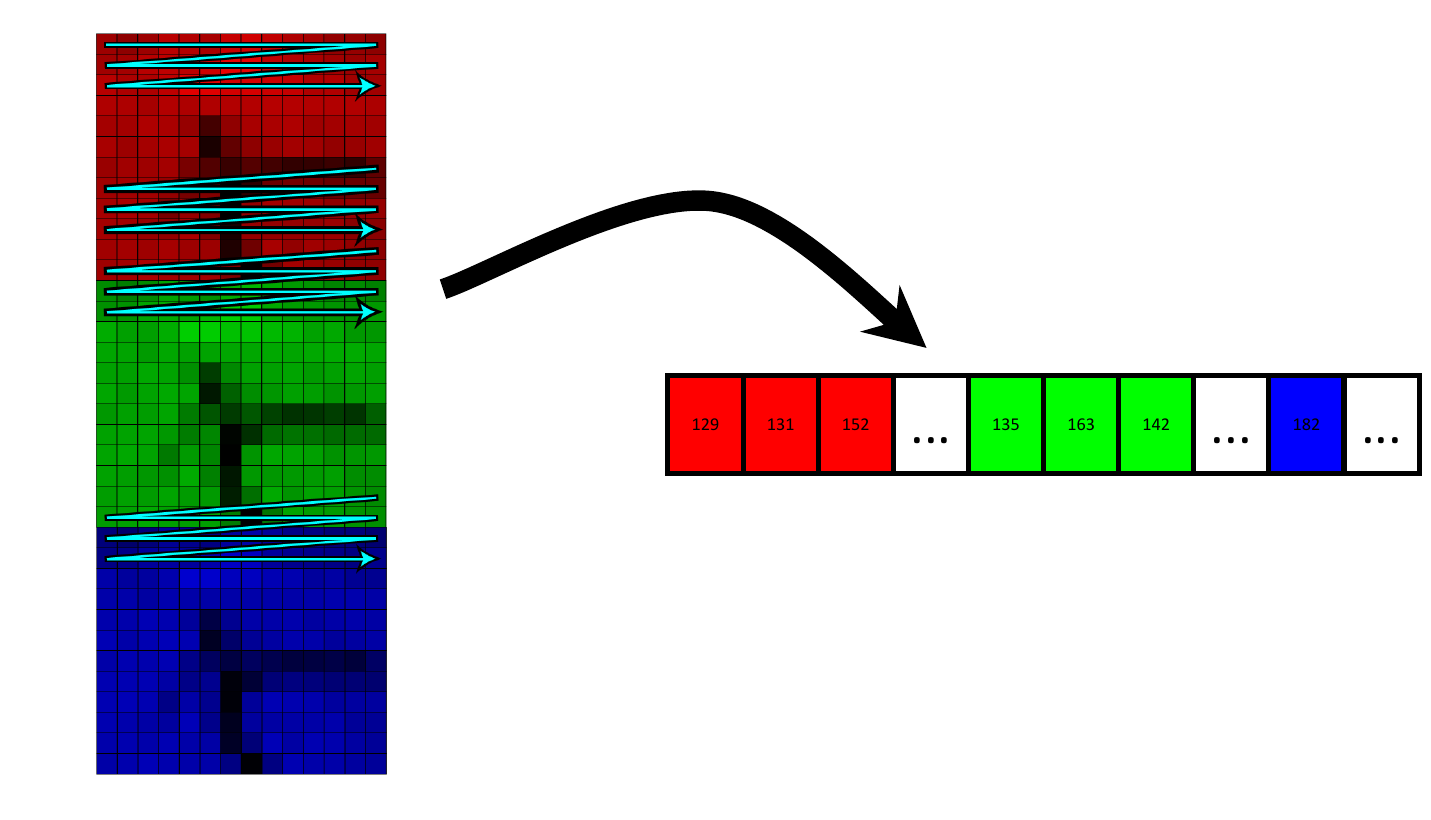
\includegraphics[width=1.2\textwidth]{./imagen14.png}
}

\frame[plain]{%
  \frametitle{¿Qué es una imagen?}
  \framesubtitle{Cuestión acerca del formato CHW}
  \begin{columns}
    \column{0.5\textwidth}
    \begin{itemize}
      \item Usaremos CHW, es lo que una gran cantidad de otras bibliotecas utilizan.
      \item En un \textcolor{blue}{array} para una imagen de $WxHxC= 1920x1080x3$, qué entrada contendría el píxel $(x,y,C)=(15,192,2)$?
      \end{itemize}
    \textcolor{red}{Fórmula: $x+y\times W + z \times W \times H$}
    \centering
  
  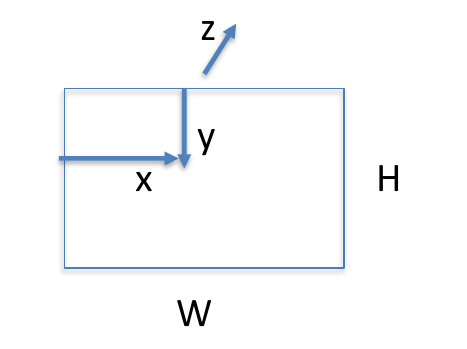
\includegraphics[width=0.5\textwidth]{./imagen16.png}
    \column{0.6\textwidth}
    \centering
  
  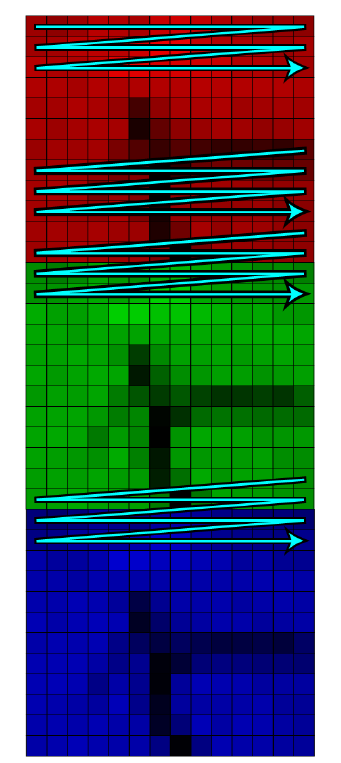
\includegraphics[width=0.5\textwidth]{./imagen15.png}

    \end{columns}
}


\frame[plain]{%
  \frametitle{¿Qué es una imagen?}
  \framesubtitle{Cuestión acerca del formato CHW}
  \begin{columns}
    \column{0.7\textwidth}
    \begin{itemize}
      \item Usaremos CHW, es lo que una gran cantidad de otras bibliotecas utilizan.
      \item En un \textcolor{blue}{array} para una imagen de $WxHxC= 1920x1080x3$, qué entrada contendría el píxel $(x,y,C)=(15,192,2)$?
      \end{itemize}
    \textcolor{red}{Fórmula: $x+y\times W + z \times W \times H$}

    \vspace{0.5cm}

    \textcolor{blue}{$15+192\times 1920 + 2 \times 1920 \times 1080 = 7833720$}

    \centering
  
  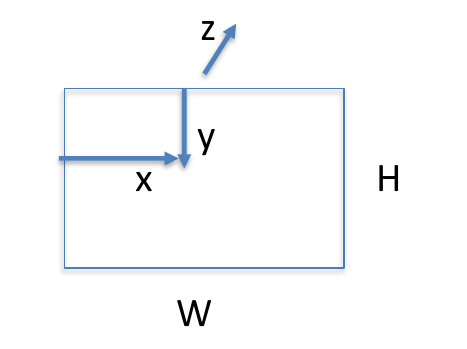
\includegraphics[width=0.5\textwidth]{./imagen16.png}
    \column{0.6\textwidth}
    \centering
  
  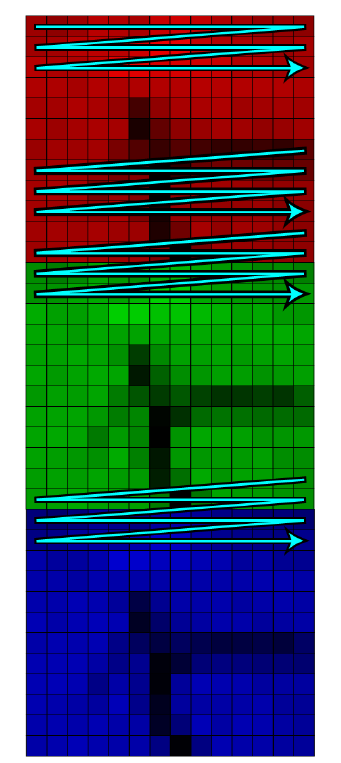
\includegraphics[width=0.5\textwidth]{./imagen15.png}

    \end{columns}
}

\frame[plain]{%
  \frametitle{¿Qué es una imagen?}
  \framesubtitle{Cuestión acerca del formato CHW}
  \begin{columns}
    \column{0.7\textwidth}
    \begin{itemize}
      \item Usaremos CHW, es lo que una gran cantidad de otras bibliotecas utilizan.
      \item En un \textcolor{blue}{array} para una imagen de $WxHxC= 1920x1080x3$, qué entrada contendría el píxel $(x,y,C)=(15,192,2)$?
      \end{itemize}
    \textcolor{red}{Fórmula: $x+y\times W + z \times W \times H$}

    \vspace{0.5cm}

    \textcolor{blue}{$15+192\times 1920 + 2 \times 1920 \times 1080 = 7833720$}

    \vspace{0.5cm}
    
    Recuerda, todo está indexado en 0 ¿Dónde va $(0,0,0)$?
    Posición $0 + 0 + 0 = 0$

    \column{0.6\textwidth}
    \centering
  
  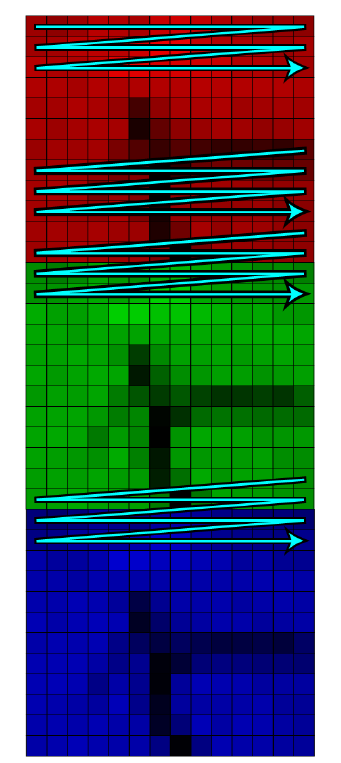
\includegraphics[width=0.5\textwidth]{./imagen15.png}

    \end{columns}
}

\frame[plain]{%
  \frametitle{¿Qué es una imagen?}
  \framesubtitle{Empleando código:}  
    \centering
  
  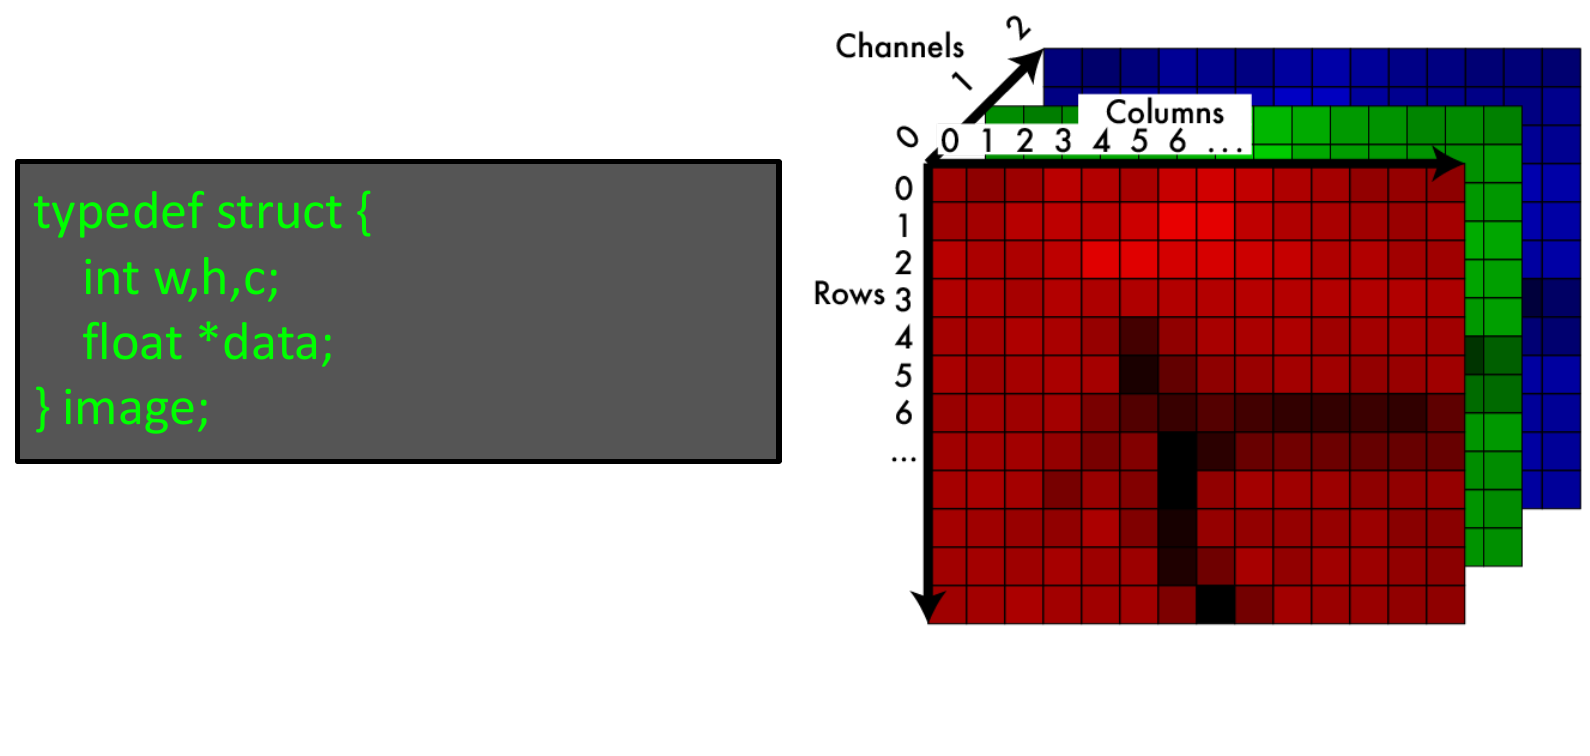
\includegraphics[width=0.9\textwidth]{./imagen17.png}

}

\frame[plain]{%
  \frametitle{¿Qué es una imagen?}
  \framesubtitle{Una imagen es un tipo de función}
  \begin{columns}
    \column{0.6\textwidth}
    \begin{itemize}
    \item Una imagen es una función bidimensional $\mathrm{Im}: \{0,1,\ldots,H-1\} \times \{0,1,\ldots,W-1\} \times \{0,1,2\} \longrightarrow \mathbb{R}$ donde $\mathrm{Im}(x,y,c)$ es la intensidad de luz en la posición $(x,y)$ del canal $c.$
    \item Nuestro objetivo es representarla empleando una función $\mathrm{Im}: \mathbb{R} \times \mathbb{R} \times \{0,1,2\} \longrightarrow \mathbb{R},$  $\mathrm{Im}(x,y,c)$ es la intensidad de luz en la posición $(x,y)$ del canal $c.$
      \end{itemize}

    \column{0.6\textwidth}
    \centering
  
  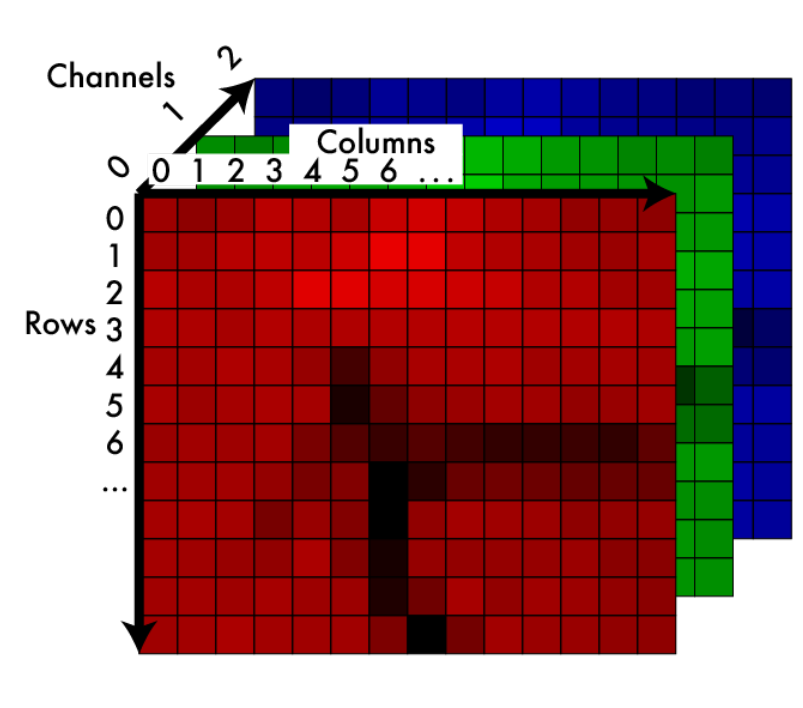
\includegraphics[width=0.7\textwidth]{./imagen9.png}

    \end{columns}
}

\frame[plain]{%
  \frametitle{¿Qué es una imagen?}
  \framesubtitle{¿Cómo se hace esta extensión?}  
    \centering
  
  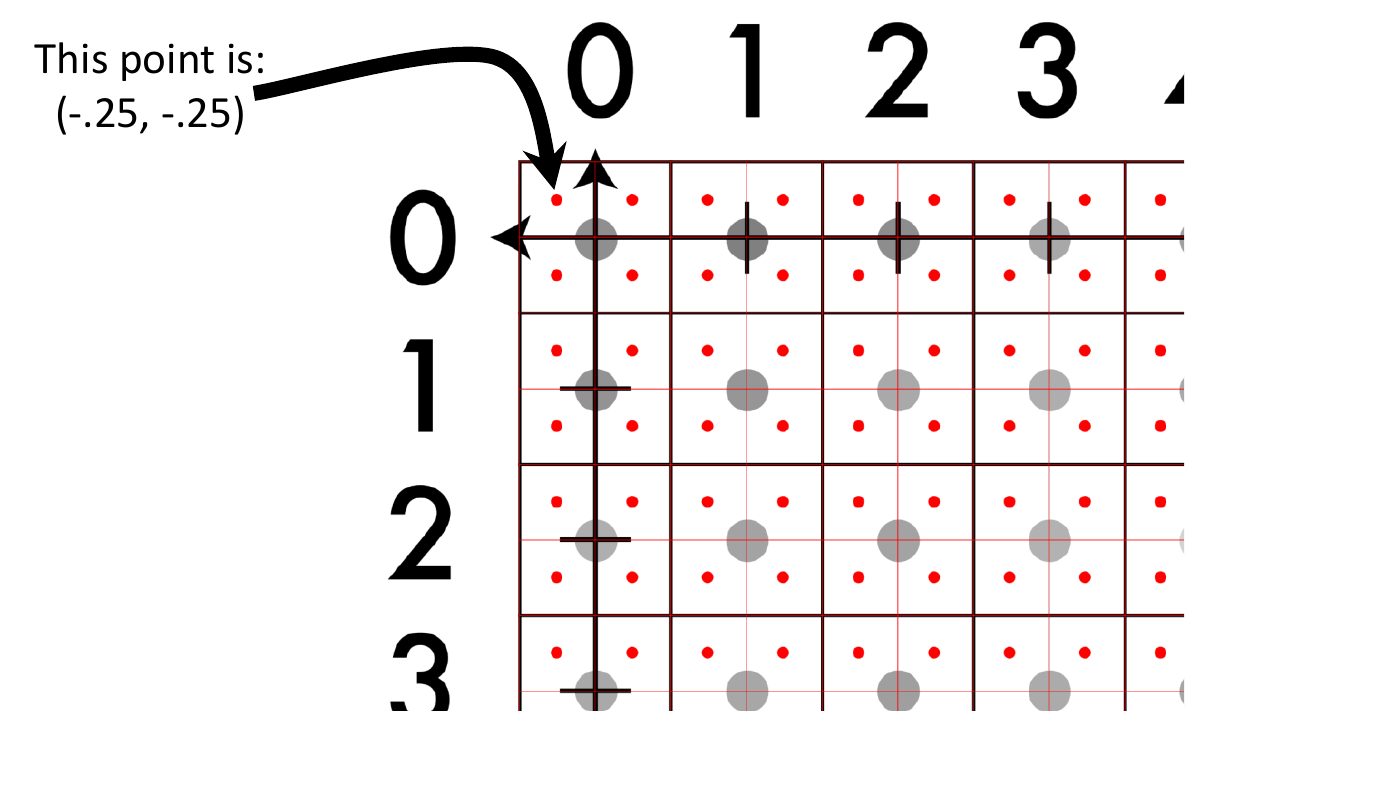
\includegraphics[width=0.9\textwidth]{./imagen18.png}

}

\frame[plain]{%
  \frametitle{¿Qué es una imagen?}
  \framesubtitle{¿Cómo se hace esta extensión?}  
\begin{itemize}
\item ¿Cómo encontramos el VALOR de una coordenada no entera, cuando la imagen solo viene con coordenadas enteros, es decir $(25,45,3)$?
\item Empleando la interpolación:
\begin{itemize} 
\item Interpolación por vecindad cercana (Nearest-Neighbor Interpolation)
\item Interpolación Bilineal
\end{itemize}
\end{itemize}
El resultado de la interpolación es una imagen continua, que es una aproximación de la imagen original:
$$
\text{Imagen}= f:\mathbb{R} \times \mathbb{R} \times \{0,1,2\} \longrightarrow \mathbb{R},
$$
donde $f(x,y,c)$ es la intensidad de luz en la posición $(x,y)$ del canal $c.$
}

\frame[plain]{%
  \frametitle{Ejemplo}
  %\framesubtitle{¿Cómo se hace esta extensión?}  
    \centering
  
  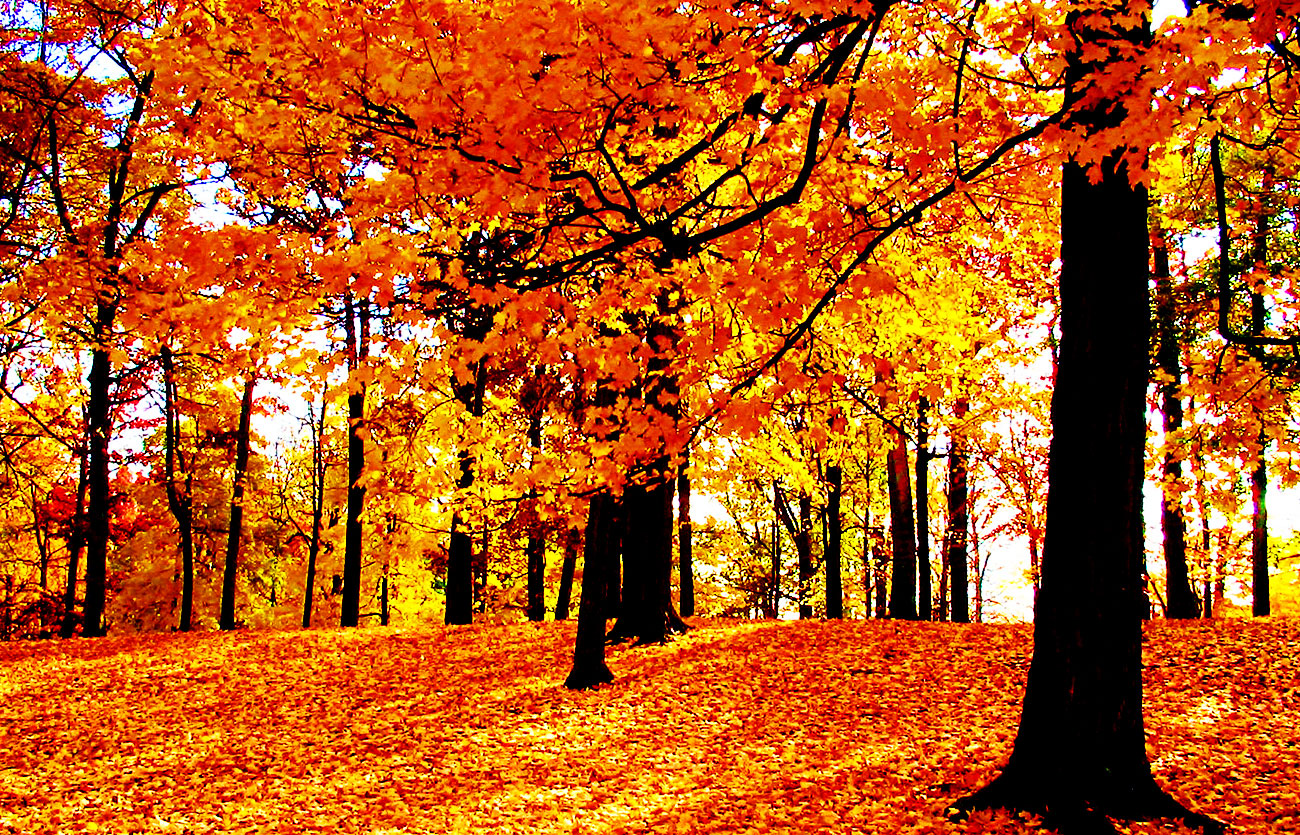
\includegraphics[width=0.9\textwidth]{./imagen.jpg}

}

\begin{frame}[fragile]
\frametitle{Código Python}
\begin{lstlisting}[language=Python]
  import numpy as np
  from matplotlib import rcParams
  import matplotlib.image as mpimg
  rcParams['figure.dpi'] = 120
  import matplotlib.pyplot as plt
  from scipy import fftpack
  img_color = plt.imread('imagen.jpg')
\end{lstlisting}  
\begin{pycode}
import numpy as np
from matplotlib import rcParams
import matplotlib.image as mpimg
rcParams['figure.dpi'] = 120
import matplotlib.pyplot as plt
from scipy import fftpack
img_color = plt.imread('imagen.jpg')
\end{pycode}  
\end{frame}

\begin{frame}[fragile]
\begin{lstlisting}[language=Python]
print("Tamano: %s" %(repr(img_color.shape)),"\n")
print("Tipo: %s" %(img_color.dtype),"\n")
print("Intensidad del pixel en la posicion 0, 0: %s" %(repr(img_color[0, 0, :])),"\n")
\end{lstlisting}
\begin{pycode}
print("Tamaño: %s" %(repr(img_color.shape)),"\n")
print("Tipo: %s" %(img_color.dtype),"\n")
print("Intensidad del pixel en la posición 0, 0: %s" %(repr(img_color[0, 0, :])),"\n")
\end{pycode}
\end{frame}

\begin{frame}[fragile]
\begin{lstlisting}[language=Python]
plt.figure(figsize=(6, 3), tight_layout=True)
plt.imshow(img_color)
plt.show()
\end{lstlisting}
\begin{pycode}
plt.figure(figsize=(6, 3), tight_layout=True)
plt.imshow(img_color)
plt.show()
\end{pycode}
\end{frame}

\frame[plain]{%
  \frametitle{Ejemplo}
  %\framesubtitle{¿Cómo se hace esta extensión?}  
    \centering
  
  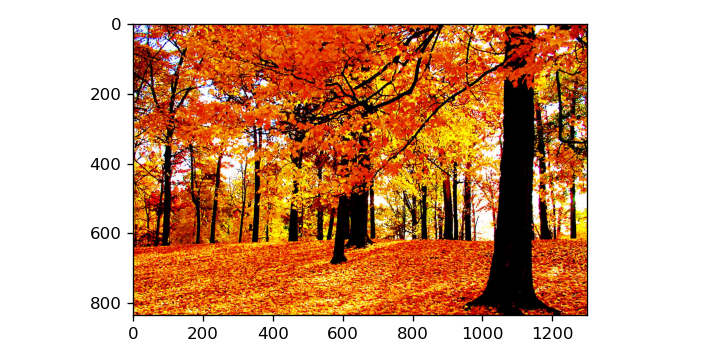
\includegraphics[width=1.1\textwidth]{./Figure_1.png}
}

\begin{frame}[fragile]
\frametitle{Ejemplo: Slicing}
\begin{lstlisting}[language=Python]
plt.figure(figsize=(6, 3), tight_layout=True)
plt.imshow(img_color[100:500, 100:200]);
plt.show()
\end{lstlisting}
\begin{pycode}
plt.figure(figsize=(6, 3), tight_layout=True)
plt.imshow(img_color[100:500, 100:200]);
plt.show()
\end{pycode}
\end{frame}

\frame[plain]{%
  \frametitle{Ejemplo: Slicing}
  %\framesubtitle{¿Cómo se hace esta extensión?}  
    \centering
  
  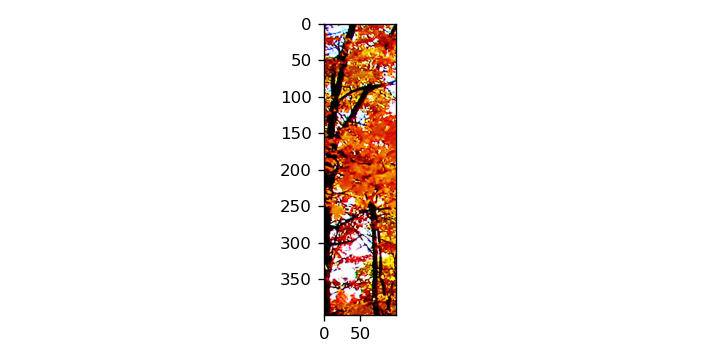
\includegraphics[width=1.1\textwidth]{./Figure_2.png}
}

\begin{frame}[fragile]
\frametitle{Ejemplo: Trasposición de imagen}
\begin{lstlisting}[language=Python]
plt.figure(figsize=(6, 3), tight_layout=True)
plt.imshow(np.transpose(img_color, axes=[1, 0, 2]));
plt.show()
\end{lstlisting}
\begin{pycode}
plt.figure(figsize=(6, 3), tight_layout=True)
plt.imshow(np.transpose(img_color, axes=[1, 0, 2]));
plt.show()
\end{pycode}
  \end{frame}
   
  \frame[plain]{%
    \frametitle{Ejemplo:  Trasposición de imagen}
    %\framesubtitle{¿Cómo se hace esta extensión?}  
      \centering
    
    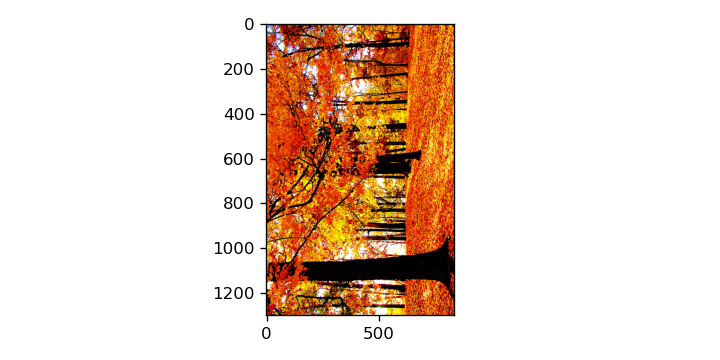
\includegraphics[width=1.1\textwidth]{./Figure_4.png}
  }


\begin{frame}[fragile]
  \frametitle{Ejemplo: Inversión de imagen}
\begin{lstlisting}[language=Python]
plt.figure(figsize=(6, 3), tight_layout=True)
plt.imshow(img_color[::-1, :, :]);
plt.show()
\end{lstlisting}
\begin{pycode}
plt.figure(figsize=(6, 3), tight_layout=True)
plt.imshow(img_color[::-1, :, :]);
plt.show()
\end{pycode}
\end{frame}
 
\frame[plain]{%
  \frametitle{Ejemplo:  Inversión de imagen}
  %\framesubtitle{¿Cómo se hace esta extensión?}  
    \centering
  
  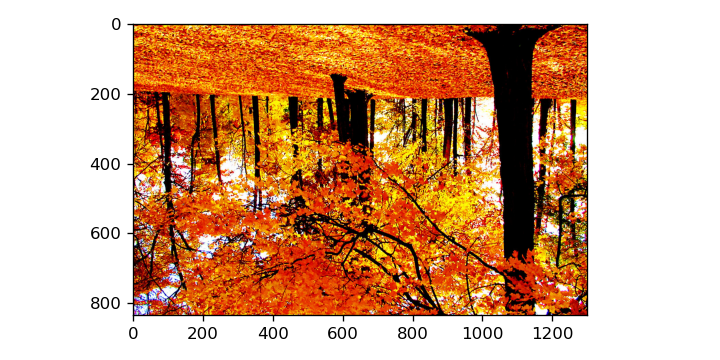
\includegraphics[width=1.1\textwidth]{./Figure_3.png}
}

\begin{frame}[fragile]
  \frametitle{Ejemplo: Espejado de imagen}
\begin{lstlisting}[language=Python]
plt.figure(figsize=(6, 3), tight_layout=True)
plt.imshow(img_color[:, ::-1, :]);
plt.show()
\end{lstlisting}
\begin{pycode}
plt.figure(figsize=(6, 3), tight_layout=True)
plt.imshow(img_color[:, ::-1, :]);
plt.show()
\end{pycode}
\end{frame}
 
\frame[plain]{%
  \frametitle{Ejemplo:  Espejado de imagen}
  %\framesubtitle{¿Cómo se hace esta extensión?}  
    \centering
  
  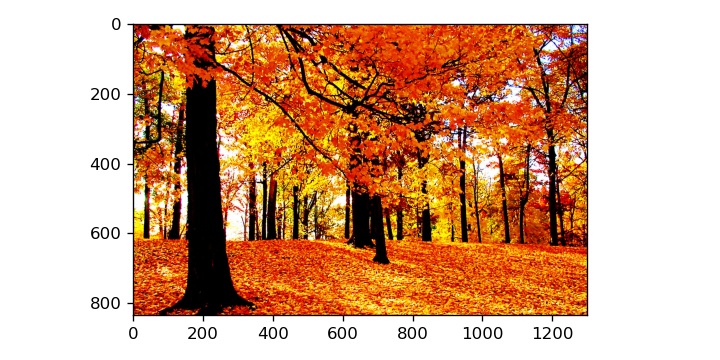
\includegraphics[width=1.1\textwidth]{./Figure_5.png}
}

\begin{frame}[fragile]
  \frametitle{Canales RGB}
La imagen empleada emplea tres canales:
\begin{lstlisting}[language=Python]
print(img_color.shape)
\end{lstlisting}
\begin{pycode}
print(img_color.shape)
\end{pycode}
\end{frame}
 

\begin{frame}[fragile]
  \frametitle{Canales RGB}
La imagen empleada emplea tres canales:
\begin{lstlisting}[language=Python]
fig, ax = plt.subplots(1, 4, figsize=(9.5, 3.2), tight_layout=True); 
ax[0].imshow(img_color[:, 350:, :])
ax[0].axis('off')
for i, color_name in enumerate(["R", "G", "B"]):
    ax[i+1].set_title(color_name)
    ax[i+1].axis('off')
    ax[i+1].imshow(img_color[:, 350:, i], cmap=plt.cm.Greys_r, vmin=0, vmax=255)
plt.show()
\end{lstlisting}
\begin{pycode}
fig, ax = plt.subplots(1, 4, figsize=(9.5, 3.2), tight_layout=True); 
ax[0].imshow(img_color[:, 350:, :])
ax[0].axis('off')
for i, color_name in enumerate(["R", "G", "B"]):
    ax[i+1].set_title(color_name)
    ax[i+1].axis('off')
    ax[i+1].imshow(img_color[:, 350:, i], cmap=plt.cm.Greys_r, vmin=0, vmax=255)
plt.show()
\end{pycode}
\end{frame}

\frame[plain]{%
  \frametitle{Canales RGB}
  %\framesubtitle{¿Cómo se hace esta extensión?}  
    \centering
  
  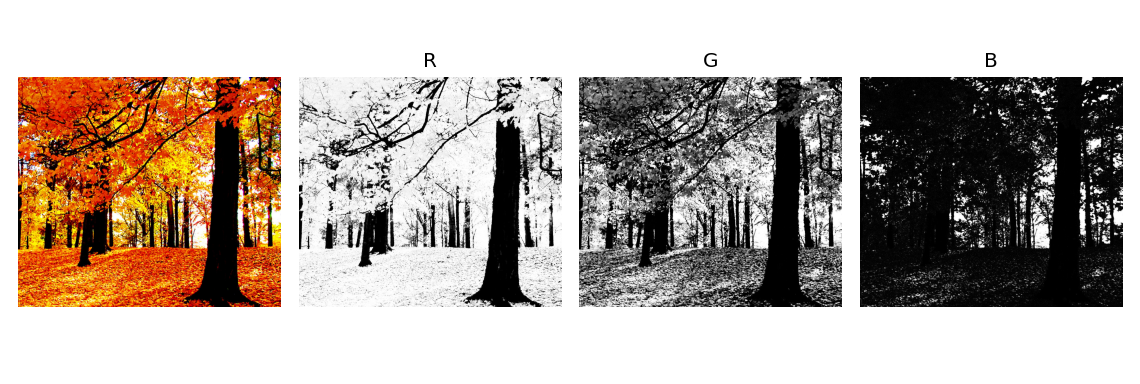
\includegraphics[width=1\textwidth]{./Figure_6.png}
}


\end{document}